\documentclass[a4paper,12pt]{article}
\usepackage{hyperref}
\usepackage{listings}
\usepackage{xcolor}
\usepackage{graphicx}


\title{\textbf{User manual for Fuse interpreter}}
\author{}
\date{}

\definecolor{codeblue}{rgb}{0.1,0.1,0.7}
\definecolor{codegreen}{rgb}{0,0.6,0}
\definecolor{codegray}{rgb}{0.5,0.5,0.5}
\definecolor{codepurple}{rgb}{0.58,0,0.82}
\definecolor{backcolour}{rgb}{0.95,0.95,0.95}

\lstdefinestyle{codestyle}{
    backgroundcolor=\color{backcolour},
    commentstyle=\color{codegreen},
    keywordstyle=\color{codeblue},
    numberstyle=\tiny\color{codegray},
    stringstyle=\color{codepurple},
    basicstyle=\ttfamily\footnotesize,
    numbers=left,
    tabsize=4
}

\lstset{style=codestyle}

\begin{document}

\maketitle

\section{Introduction}
This document describes how to use Fuse interpreter. The interpreter supports custom syntax and allows debugging of programs written for it. Configuration files define the syntax and instruction names, providing flexibility in operation.

\section{Features}
\begin{itemize}
	\item Supports 32-bit integer variables.
	\item Configurable syntax for instructions via settings files.
	\item Built-in debugging mode.
	\item Supports both unary and binary operations.
	\item Preserves configuration across sessions.
	\item Handles single-line and multi-line comments in input files.
	\item Memory-efficient variable storage using a trie data structure.
\end{itemize}

\newpage

\section{Usage Instructions}

\subsection{Running the Interpreter}
To run the interpreter, execute the following command:
\begin{lstlisting}[language=bash]
$ fuse [options]
\end{lstlisting}
\begin{itemize}
	\item \texttt{-f <input\_file>}: Specify program input file.
	\item \texttt{-c <config\_file>}: Specify configuration file.
	\item \texttt{--base\_input <base>}: Specify counting system base for input.
	\item \texttt{--base\_output <base>}: Specify counting ststem for output.
	\item \texttt{--base\_assign <base>}: Specify counting system for assignations.
	\item \texttt{--debug}: Enable debugging mode.
	\item \texttt{-d}: Enable logging system-user interaction.
	\item \texttt{-s}: Enable silent mode. Doesn't generate logs.
	\item \texttt{-t}: Preserve saving temporary files.
	\item \texttt{-m}, \texttt{--menu}: Start interactive menu.
	\item \texttt{-h}, \texttt{--help}: Displays help information.
	\item \texttt{-i}, \texttt{--info}: Displays creator information.
	\item \texttt{-v}, \texttt{--version}: Displays Fuse version.
\end{itemize}



\subsection{Supported Operations}
\begin{itemize}
	\item \textbf{Unary Operations:}
	      \begin{itemize}
		      \item \texttt{not}: Bitwise NOT.
		      \item \texttt{input}: Reads a value from standard input.
		      \item \texttt{output}: Writes a variable value to standard output.
	      \end{itemize}
	\item \textbf{Binary Operations:}
	      \begin{itemize}
		      \item \texttt{add}: Addition.
		      \item \texttt{sub}: Subtraction.
		      \item \texttt{mult}: Multiplication.
		      \item \texttt{div}: Integer division.
		      \item \texttt{rem}: Remainder.
		      \item \texttt{pow}: Modular exponentiation.
		      \item \texttt{and}, \texttt{or}, \texttt{xor}: Bitwise operations.
	      \end{itemize}
\end{itemize}

\subsection{Configuration File Format}
The configuration file defines the mapping of commands and syntax. It supports single-line comments starting with \texttt{\#}. Example:
\begin{lstlisting}
right= # this is a comment
(div)
add sum
[sub minus
pow ^ and it is a comment...]
xor <>
xor ><
#xor <>
output print
= ->
\end{lstlisting}


\subsection{Input File Format}
The input file contains program instructions, with commands separated by \texttt{;} and optional spaces or newlines. Example:
\begin{lstlisting}
var_1 = 1F4;
var_2 = mult(var_2, 4);
Var3 = add(div(var_2, 5), rem(var_1, 2));
print(Var3);
\end{lstlisting}

\newpage


\section{Interactive menu}
If you doesn't specify any cli options, or pass \texttt{-m} flag interactive menu will start. It can configure interpreter and run the program. Example usage: \\

\begin{center}
	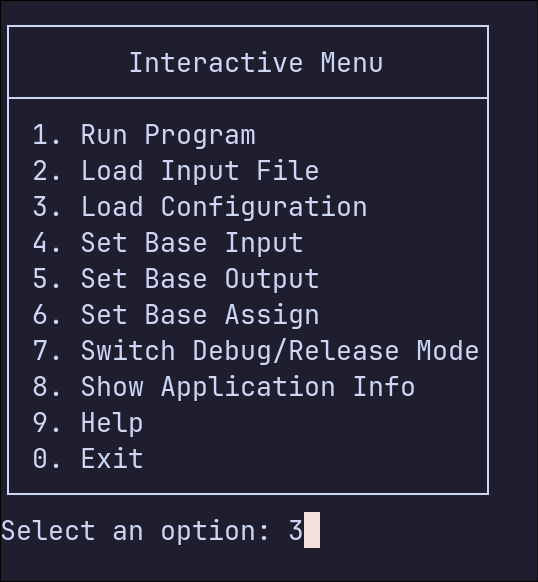
\includegraphics[width=0.5\textwidth]{assets/menu.png}
\end{center}


\section{Debugging Mode}
To enter debugging mode, use the \texttt{--debug} flag. When the interpreter encounters a \texttt{\#BREAKPOINT} comment, it pauses execution and allows interactive debugging.


\subsection{Interactive Commands}
In debugging mode, you can:
\begin{itemize}
	\item View variable values in hexadecimal and binary.
	\item List all known variables.
	\item Modify or declare new variables.
	\item Delete variables.
	\item Exit debugging mode or terminate the interpreter.
\end{itemize}

\newpage

Example interaction:
\begin{center}
	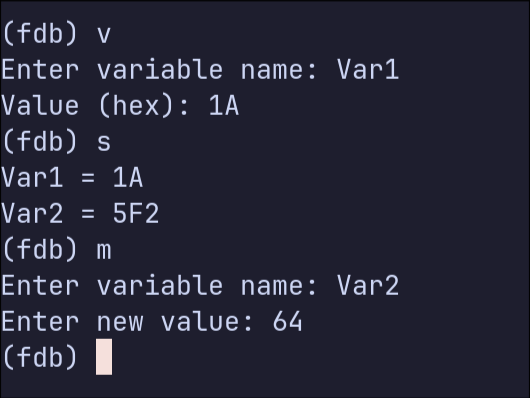
\includegraphics[width=0.5\textwidth]{assets/debugger.png}
\end{center}

\section{Error Handling}
The interpreter detects and reports runtime errors, such as:
\begin{itemize}
	\item Invalid operations or syntax.
	\item Undefined variable usage.
	\item Invalid configuration settings.
\end{itemize}

\section{Conclusion}
This interpreter provides a robust and flexible tool for executing programs with customizable syntax and debugging support. Utilize the configuration and debugging features to tailor the interpreter to your needs.
\vspace*{\fill}

\begin{center}Created in \raisebox{-0.5ex}{
\includegraphics[height=1em]{assets/linux.png}} \& \raisebox{-0.5ex}{
\includegraphics[height=1em]{assets/neovim.png}}
	with \raisebox{-0.5ex}{
\includegraphics[height=1em]{assets/love.png}}\end{center}

\end{document}
